
\begin{figure}
\def\layersep{2.0cm}
\centering
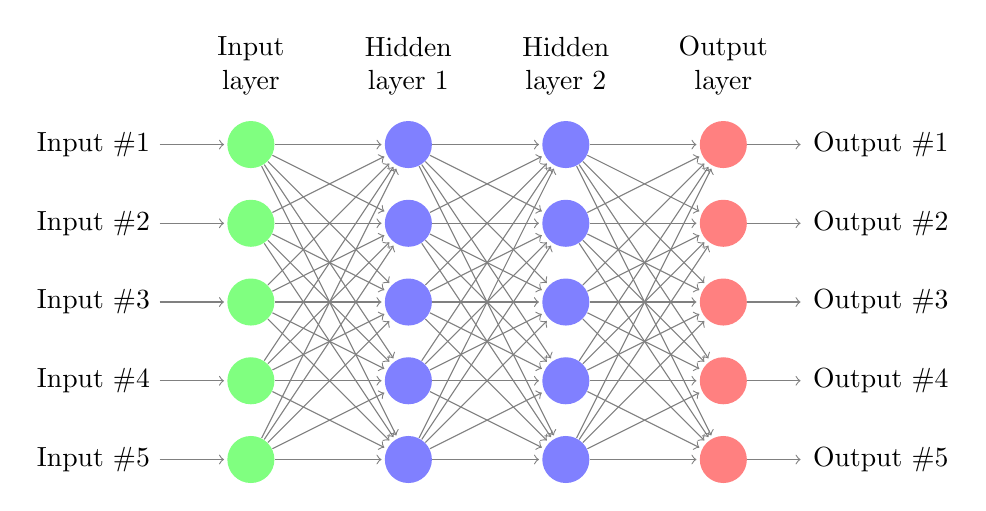
\begin{tikzpicture}[shorten >=1pt,->,draw=black!50, node distance=\layersep]
\tikzstyle{every pin edge}=[<-,shorten <=1pt]
\tikzstyle{neuron}=[circle,fill=black!25,minimum size=17pt,inner sep=0pt]
\tikzstyle{input neuron}=[neuron, fill=green!50];
\tikzstyle{output neuron}=[neuron, fill=red!50];
\tikzstyle{hidden neuron}=[neuron, fill=blue!50];
\tikzstyle{annot} = [text width=4em, text centered]

% Write input labels
\foreach \name / \y in {1,...,5}
\node (IL-\name) at (0,-\y) {Input \#\y};

% Draw the input layer nodes
\foreach \name / \y in {1,...,5}
\node[input neuron, right of=IL-\name] (I-\name) {};

\foreach \source in {1,...,5}
\path (IL-\source) edge (I-\source);

% Draw the hidden layer nodes
\foreach \name / \y in {1,...,5}
\node[hidden neuron, right of=I-\name] (H1-\name) {};

% Draw the hidden layer nodes
\foreach \name / \y in {1,...,5}
\node[hidden neuron, right of=H1-\name] (H2-\name) {};

% Draw the output layer nodes
\foreach \name / \y in {1,...,5}
\node[output neuron, right of=H2-\name] (O-\name) {};

%Write output labels
\foreach \name / \y in {1,...,5}
\node[right of=O-\name] (OL-\name) {Output \#\y};

\foreach \source in {1,...,5}
\path (O-\source) edge (OL-\source);

% Connect every node in the hidden layer with the output layer
\foreach \source in {1,...,5}
\foreach \dest in {1,...,5}
\path (I-\source) edge (H1-\dest);

\foreach \source in {1,...,5}
\foreach \dest in {1,...,5}
\path (H1-\source) edge (H2-\dest);

\foreach \source in {1,...,5}
\foreach \dest in {1,...,5}
\path (H2-\source) edge (O-\dest);

%Annotate the layers
\node[annot,above of=O-1, node distance=1cm] {Output layer};
\node[annot,above of=I-1, node distance=1cm] {Input layer};
\node[annot,above of=H1-1, node distance=1cm] {Hidden layer 1};
\node[annot,above of=H2-1, node distance=1cm] {Hidden layer 2};

\end{tikzpicture}
\caption{Multi-layer perceptron}
\label{multilayerperceptron}
\end{figure}